\section{Adaptive-precision ADC Design}\label{architecture}

This section presents the proposed adaptive-precision ADC design. Targeting image processing applications, we consider SS and SAR/SS ADCs, which are suitable for image sensor integration. 
Section~\ref{over1} and \ref{over2} provide architecture overview of SS and SAR/SS ADCs. 
Section~\ref{gating1} presents the proposed power gating method. 
Section~\ref{gating2} and \ref{gating3} present adaptive-precision tuning of SS and SAR/SS ADCs. The key characteristics of the proposed adaptive-precision ADC architecture are summarized 
as follows. 

%The basic modules of the two ADC designs is overviewed firstly in \ref{over1} and \ref{over2}. Then, after showing the power gating implementation in \ref{gating1}, the adaptive-precision tuning within SS and SAR/SS ADCs is specifically described in \ref{gating2} and \ref{gating3}, with the following architectural enhancements:

\begin{enumerate}[\IEEEsetlabelwidth{3)}]
	\item 
	The thermometer-code counter in SS ADC is extended to support high/low-precision modes for adaptive-precision conversion, which can also provide an exponentially long window of opportunity for power gating.
	\item
    Stability-optimizing switches are inserted into the comparators in SS ADC to avoid unpredictable latch for low-precision conversion due to comparator power off. 
    \item
    Additional control signals in SAR/SS ADC are carefully reused and effectively minimized, enabling efficient power-scaling capabilities with limited numbers of shared level-shifters and inverters.      
\end{enumerate} 


%For other ADCs of different architecture, the proposed method can also be adopted.

\subsection{SS ADC Architecture Overview}\label{over1}

The overall architecture of SS ADC is presented in Fig.~\ref{SSADC}. The main modules include column-parallel correlated double sampling (CDS) circuits, comparators, 
and a column-shared ramp generator. Fig.~\ref{SSWAVE} shows the operational waveform of SS ADC. When the ramp signal exceeds the output of the CDS circuit in a specific column, 
the corresponding comparator is flipped and latches the time information $\Delta t$ into the following 8-bit latch as the conversion results. 
Such conversions across all columns is done as soon as the ramp signal reaches $V_{refh}$.

\begin{figure}[htbp]
	\centerline{\includegraphics[width=3.5in]{./Figures/SSADC.eps}}
	\caption{The overall architecture of SS ADC.}
	\label{SSADC}
\end{figure} 

\begin{figure}[htbp]
	\centerline{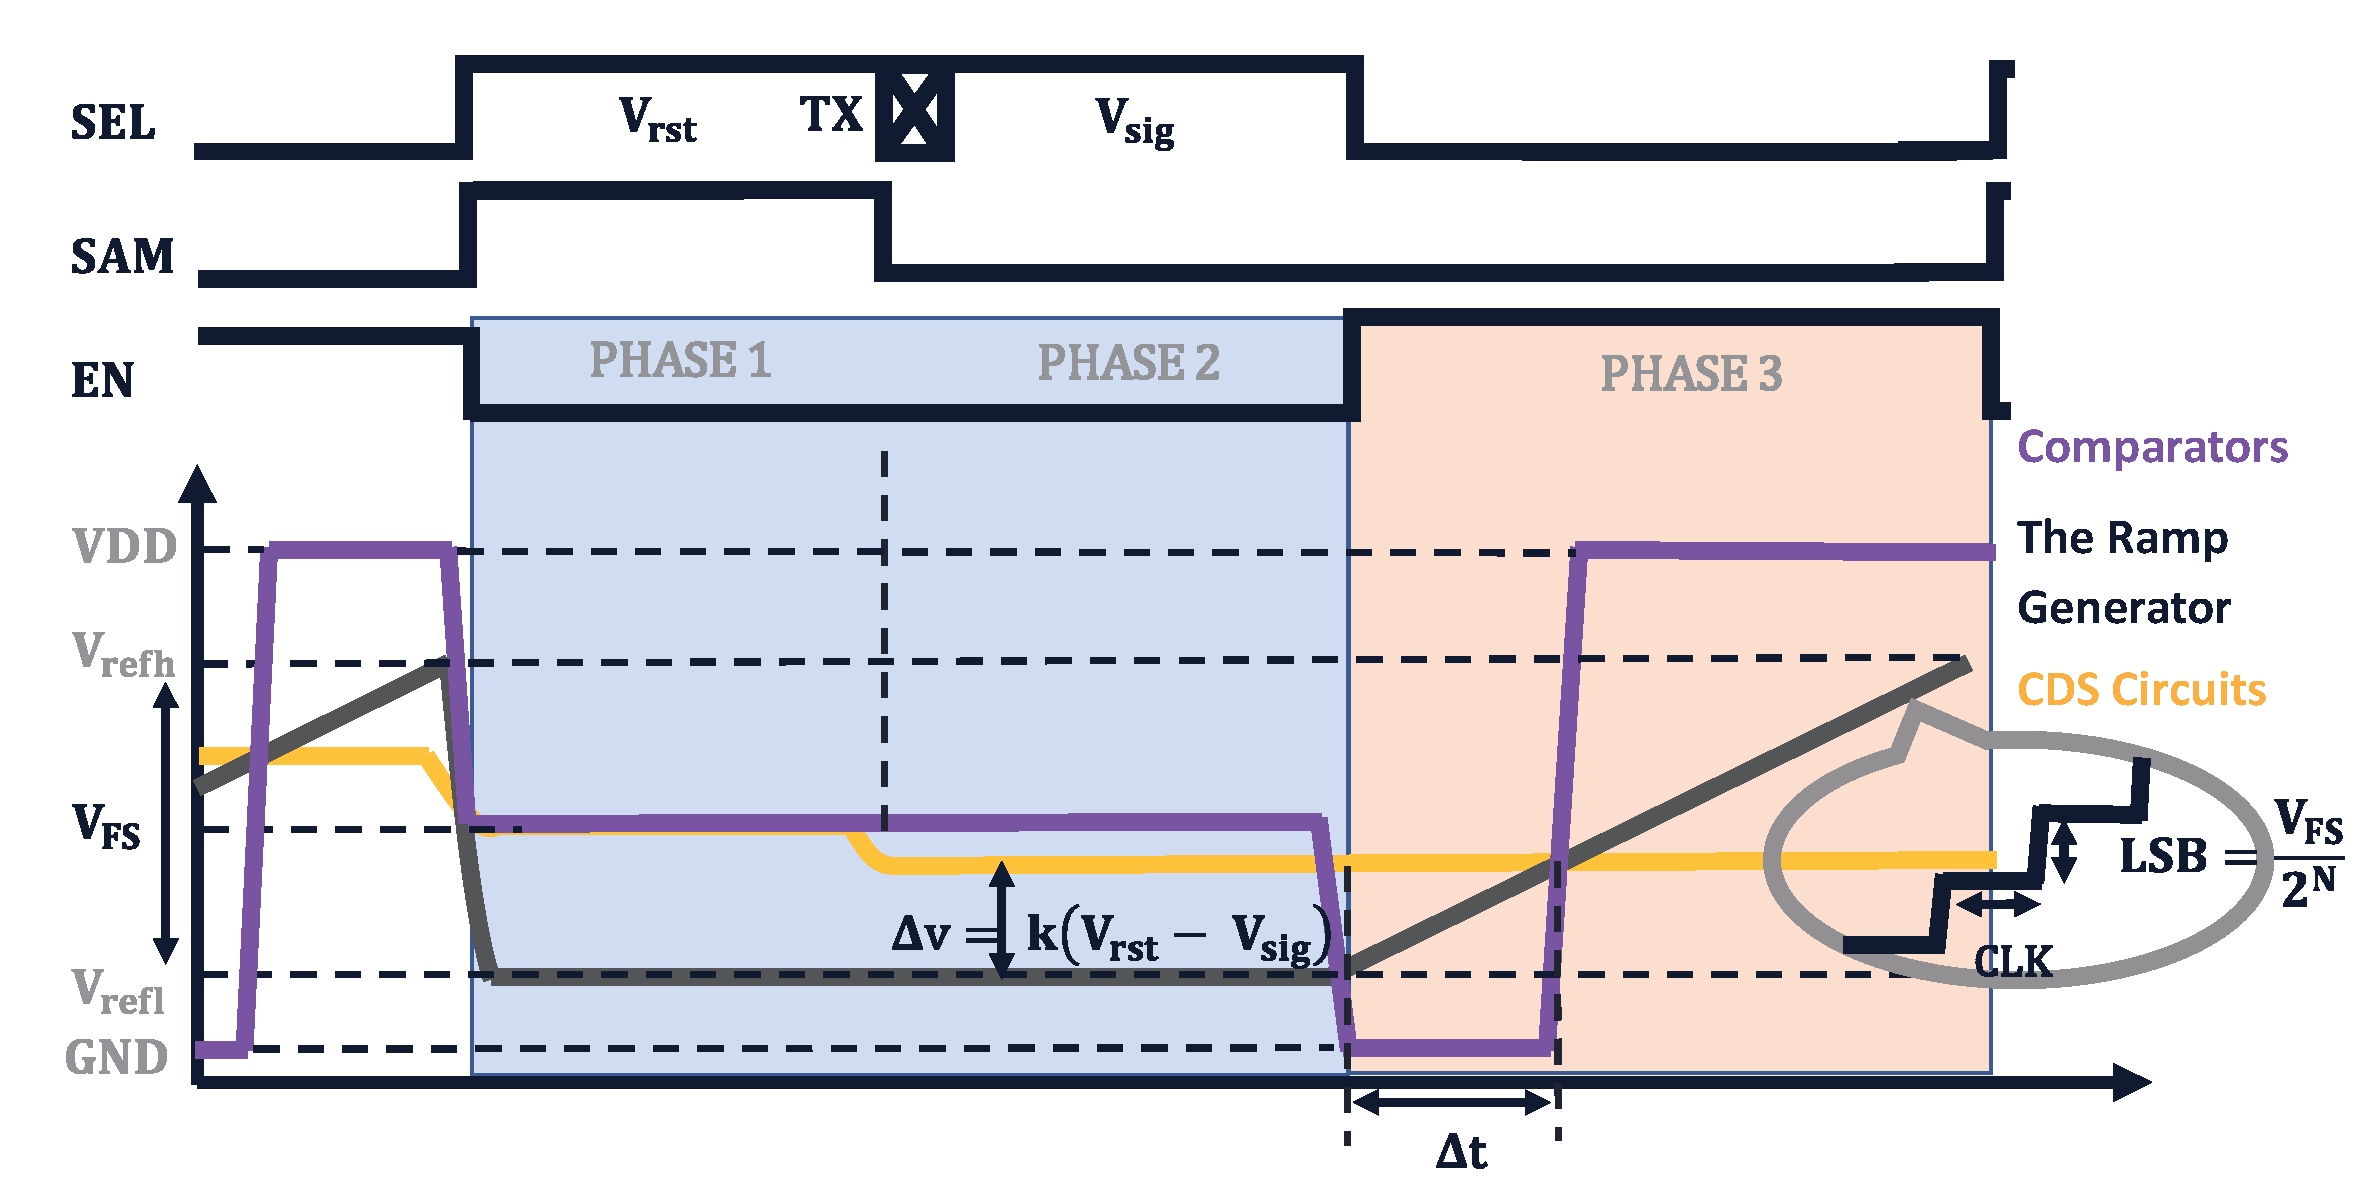
\includegraphics[width=3.5in]{./Figures/SSWAVE.eps}}
	\caption{The operational waveform of SS ADC.}
	\label{SSWAVE}
\end{figure}

Next, we describe the circuit structure of the key modules in detail. 

\subsubsection{CDS Circuits}

CDS circuits are the interface between pixel array and ADC, responsible for subtracting the pixel signal voltages 
from reference voltages and amplifying the difference by a certain coefficient. The difference (i.e. $\Delta{V}$ 
in Fig.~\ref{SSWAVE}) is physically attached to the exposure time of the pixels, and subtraction helps remove the 
noise caused by the varying reference voltages. 

Switched-capacitor operational amplifiers are commonly used in CDS circuits (shown in Fig.~\ref{CDS}). According to the law of charge conservation, 
the output voltage of the CDS circuits (in PHASE2 of Fig.~\ref{SSWAVE}) can be calculated as \eqref{eq1}, consistent with the requirements. Input offset cancellation (IOS) is also implemented~\cite{razavi_design_1992}, 
which is necessary because the amplifiers in different columns may have different offset voltages.

\begin{figure}[htbp]
	\centerline{\includegraphics[width=2.5in]{./Figures/CDS.eps}}
	\caption{The structure of the CDS circuits.}
	\label{CDS}
\end{figure} 

\begin{equation}
	\begin{aligned}
		V_{out}&=\left[ V_{ref}+\frac{C_1}{C_2}\ast\left(V_{rst}-V_{sig}\right)\right]\ast\frac{\beta A}{1+\beta A}\\
		&\;{+}\;\left(V\right._{refl}+V_{os})\ast\frac{A}{1+A}\ast\frac{1}{\beta A}\\
		&\;where\ \ \beta=\frac{C_2}{C_1+C_2}
		\label{eq1}
	\end{aligned}
\end{equation}

\subsubsection{Ramp Generator}

As shown in Fig.~\ref{RAMP}, the ramp generator in SS ADC consists of a thermometer-code counter and a capacitor digital-to-analog converter (CDAC). 
While the capacitors in CDAC are being switched one by one from $V_{refl}$ to $V_{vefh}$, the output voltage of the ramp generator is expressed as \eqref{eq2} according to the law of charge conservation. 
In this equation, $N$ represents the number of switched capacitors and $M$ represents the total number of capacitors with the same size (for the 8-bit precision, the total number will be 255). 
Therefore, in PHASE3 (shown in Fig.~\ref{SSWAVE}), the ramp signal changes in stages from $V_{refl}$ to $V_{refh}$, of which the range matches the output of CDS circuits. 
The height of each stage is the least significant Bit (LSB) of the ADC conversion.

The three buffers shown in Fig.~\ref{RAMP} ensure that the reference voltages and ramp signal have sufficient driving capabilities, 
and the output buffer has the largest size in order to drive hundreds of column-parallel comparators.

\begin{figure}[htbp]
	\centerline{\includegraphics[width=3.5in]{./Figures/RAMP.eps}}
	\caption{The structure of the ramp generator in SS ADC.}
	\label{RAMP}
\end{figure} 

\begin{equation}
	V_{ramp}=V_{refl}+\frac{N}{M}\ast\left(V_{refh}-V_{refl}\right)
	\label{eq2}
\end{equation}

\subsubsection{Comparators}

The comparators are used to compare the CDS circuit output with the ramp signal from the ramp generator. 
In SS ADC, two-stage open-loop comparators can be applied as shown in Fig.~\ref{COM}. According to the law of charge conservation, 
the comparator output (PHASE3 shown in Fig.~\ref{SSWAVE}) can be computed as \eqref{eq3}. The comparison is dominated by $V_{ramp}-V_{cds}$ as long as the amplifiers’ open-loop gain 
is large enough while the IOS is also realized.% In addition, the comparators’ speed relies on the bandwidth and slew rate of the amplifiers.

\begin{figure}[htbp]
	\centerline{\includegraphics[width=2.5in]{./Figures/COM.eps}}
	\caption{The structure of the comparators in SS ADC.}
	\label{COM}
\end{figure} 

\begin{equation}
	\begin{aligned}
		V_{out}&=A^2(V_{ramp}-V_{cds})\\
		&\;{+}\;\left(V_{refl}+V_{os}\right)\ast\frac{A}{1+A}\\ 		
		\label{eq3}
	\end{aligned}
\end{equation}

\subsection{SAR/SS ADC Architecture Overview}\label{over2}

%Fig.~\ref{SARADC} shows 
The overall architecture of SAR/SS ADC is similar to that of SS ADC shown in Fig.~\ref{SSADC}. The key differences are that the comparators are replaced by low-precision (4bit) SAR sub-ADC, and
the ramp generator is replaced by a resistor digital-to-analog converter (RDAC) with a one-hot code counter.

\iffalse
\begin{figure}[htbp]
  \centerline{\includegraphics[width=3.5in]{./Figures/SARADC.eps}}
  \caption{Overall architecture of SAR/SS ADC.}
  \label{SARADC}
  \end{figure}
\fi 

As shown in Fig.~\ref{SAR}, a SAR sub-ADC is composed of two input buffers of the reference voltages, an array of digital-to-analog capacitors, a dynamical comparator and a SAR logic block. While generating the upper 4-bit results, $V_{X}$ in SAR sub-ADC is changed according to SAR logic. That means after 4 comparisons 
with the reference voltage, $V_{X}$ is equal to \eqref{eq4}, where $D_{U}\left[\,i\,\right]$ is the $i$ th bit of the upper 4 bits. 
Then the ramp generator starts working, $V_{X}$ then increases gradually as \eqref{eq5}, where $D_{L}\left[\,i\,\right]$ is the $i$ th bit of the lower 6 bits. 
At the time when $V_{X.2}$ exceeds $V_{ref}$, the corresponding $V_{cds}$ is expressed as \eqref{eq6}, which can be represented by the 10-bit conversion results, exactly.

\begin{figure}[htbp]
	\centerline{\includegraphics[width=3in]{./Figures/SAR.eps}}
	\caption{The structure of SAR sub-ADCs in SAR/SS ADC.}
	\label{SAR}
\end{figure}

\begin{equation}
	V_{X.1}=V_{cds}+\sum_{i=1}^{4} {\frac{V_{ref}}{2^{i}}\ast{D_{U}\left[\,i\,\right]}}
	\label{eq4}
\end{equation}

\begin{equation}
	\begin{aligned}
		&V_{X.2}=V_{X.1}+\frac{V_{ramp}}{2^4}\\ &where\  V_{ramp}=\frac{V_{ref}}{2^6-1}\ast\sum_{i=1}^{6}2^{6-i}\ast{D_{L}\left[\,i\,\right]}
		\label{eq5}
	\end{aligned}	
\end{equation}

\begin{equation}
	\begin{aligned}
		&V_{cds}=k\ast(V_{rst}-V_{sig})\\
		&\;{\approx}\;{V_{ref}-\sum_{i=1}^{4} \frac{V_{ref}}{2^{i}}\ast{D_{U}\left[\,i\,\right]}-\sum_{i=1}^{6} \frac{V_{ref}}{2^{4+i}}\ast{D_{L}\left[\,i\,\right]}}
		\label{eq6}
	\end{aligned}
\end{equation}

It is worth noting that we assign 14 steps for the 4 comparisons with SAR logic (in SAR/SS ADC, we define 1 clock step as 2 clock periods, which is 100ns). Both the first and second comparison takes 4 steps and the following two comparison takes 3 steps. It is because that the more rapidly $V_{X}$ can be changed, the more time it may be required for comparison. As for the last comparison with SS logic, 1 step is sufficient because $V_{X}$ will not exceed $V_{ref}$ rapidly, allowing the comparators to response in-time.

Fig.~\ref{RRAMP} shows the structure of the ramp generator in SAR/SS ADC, which consists of an R-string made up of 68 unit resistors. $V_{ramp}$ has a total number of 68 steps,
of which 64 steps with a step size of $(V_{refh}-V_{refl})/64$ are used to generate the lower 6-bit results and 4 redundant steps are used to ensure that the comparators 
will always be flipped to latch the results. During operation, $V_{0}$ to $V_{67}$ in the ramp generator is sequentially selected as the output and thereby 
$V_{ramp}$ is changed from $V_{vefl}$ to $V_{vefl}+17/16(V_{refh}-V_{refl})$.

\begin{figure}[htbp] 
	\centerline{\includegraphics[width=2.5in]{./Figures/RRAMP.eps}}
	\caption{The structure of the ramp generator in SAR/SS ADC.}
	\label{RRAMP}
\end{figure}

Compared to CDAC, RDAC is able to generate the ramp signal without the gain error caused by the input capacitors of the output buffer, 
which is necessary to achieve 10-bit precision in SAR/SS hybrid architecture.
Besides, the two buffers of the reference voltages in the RDAC require less energy than those in the CDAC due to less load capacitance.  

The related operational waveform of SAR/SS ADC is shown in Fig.~\ref{SARWAVE}. The upper 4-bit results (as the second last item of \eqref{eq6}) are generated 
with SAR logic and the lower 6-bit results (as the last item of \eqref{eq6}) are counted according to the time between the ramp signal’s start and the comparators’ last flip. 

\begin{figure}[htbp]
	\centerline{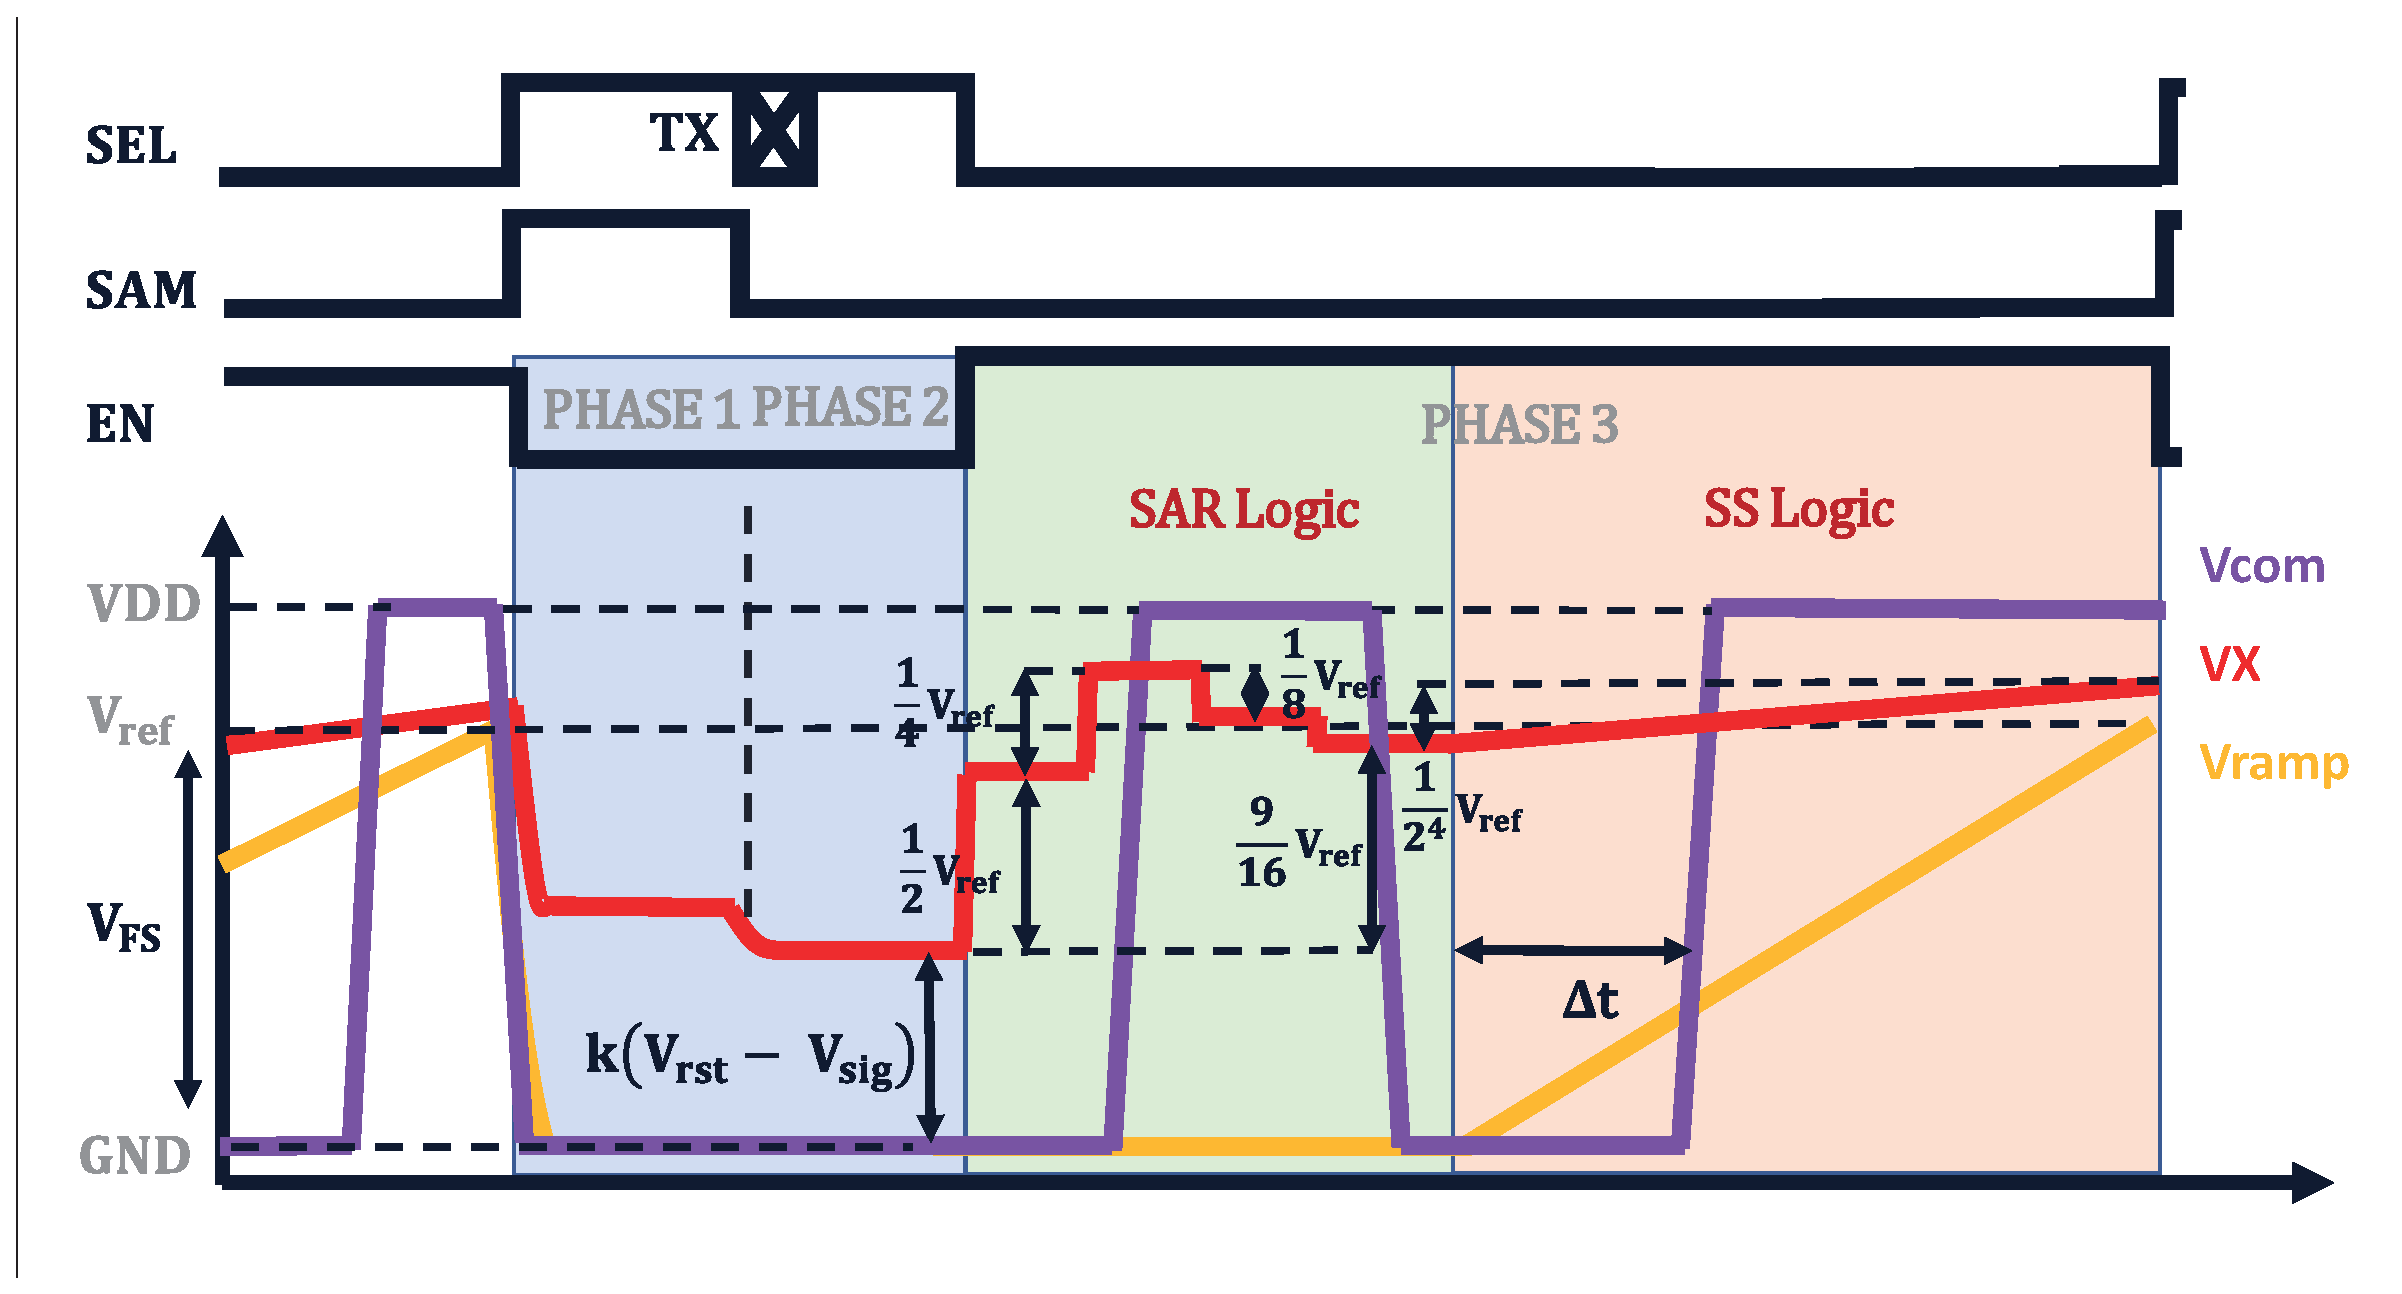
\includegraphics[width=3.5in]{./Figures/SARWAVE.eps}}
	\caption{The operational waveform of SAR/SS ADC.}
	\label{SARWAVE}
\end{figure} 

As for the dynamical comparators inside SAR sub-ADC, a strong-arm comparator with pre-amplifiers can be used as shown in Fig.~\ref{LATCH}. Such comparators 
are suitable for multiple comparisons because high speed is easily achieved and every comparison is under the control of the clock. Besides, the offset voltages of the pre-amps can be effectively eliminated by output offset cancellation (OOS) \cite{razavi_design_1992}.

\begin{figure}[htbp]
	\centerline{\includegraphics[width=3.5in]{./Figures/LATCH.eps}}
	\caption{The structure of the comparators in SAR sub-ADCs.}
	\label{LATCH}
\end{figure} 

The design decision regarding 4/8-bit adaptive-precision for SS ADC and 4/10-bit adaptive-precision for SAR/SS ADC is discussed in Sect.~\ref{discussion}.

%\subsection{Power Gating and Adaptive-Precision Implementation}\label{strategy}

\subsection{Implementation of Power Gating}\label{gating1}

As shown in  Fig.~\ref{GATING}, the proposed power gating method is implemented by adding PMOS-transistor switches between the functional blocks and the supply voltage \cite{keating_low_2007}. 
When the switches are turned off, the corresponding blocks’ current paths are cut off and the energy is saved. 

Fine-grain power gating is beneficiary to power and energy savings. On the other hand, 
to avoid unacceptable IR drop, the area overhead of the switch circuit may be significant, 
and inverters need to be inserted between the control signal and the switching gates for 
sufficient driving capabilities. 

In addition, the longer the functional blocks is powered off, the better power scaling benefit can be obtained. Therefore, for power gating, continuous long periods of time are preferred than individual short periods of time, since block shutdown and recovery times should also be considered.
As shown in Fig.~\ref{TIME}, due to the shutdown and recovery time of the function block, frequent 
power gating over short time intervals may introduce extra overhead. 

Since column-parallel ADC not only has high column-parallel current that can be controlled, but also offers continuously and exponentially long power-off time intervals thanks to the widely adopted SS conversion logic, applying power gating to this architecture is highly efficient.

\begin{figure}[htbp]
	\centerline{\includegraphics[width=3.5in]{./Figures/GATING.eps}}
	\caption{Implementation of power gating.}
	\label{GATING}
\end{figure} 

\begin{figure}[htbp]
	\centerline{\includegraphics[width=3.5in]{./Figures/TIME.eps}}
	\caption{Continuous long time versus separated short time for power gating.}
	\label{TIME}
\end{figure}  

\subsection{Adaptive-Precision Implementation for SS ADC}\label{gating2}

As evaluated in Sect.~\ref{result}, SS ADC power consumption is mainly contributed by column-parallel comparators, bias circuits, and output the buffer of ramp generator. 
Considering that all bias circuits are settled down only once (tens of microseconds after the whole system is powered up) and then other circuits can be settled down quickly by the distributed 
bias circuits, it is only necessary to apply power gating to the amplifiers in the comparators and the output buffer in the ramp generator.

For low-precision conversion, the thermometer-code counter should be extended to support switching the capacitors in CDAC 16 by 16 instead of one by one and thereby the ramp signal can reach $V_{refh}$ in 16 steps (for 4 bits) instead of in 256 steps (for 8 bits). 
After the 16 steps, comparators and output buffer can be powered off for an extended period of time, leaving the related signals decrease gradually.
The related waveform is shown in Fig.~\ref{SS_pg}. 

\begin{figure}[htbp]
	\centerline{\includegraphics[width=3.2in]{./Figures/SS_pg.eps}}
	\caption{Adaptive-precision and power gating implementation for SS ADC.}
	\label{SS_pg}
\end{figure} 

To avoid the decreasing comparator outputs causing extra latches for the low-precision conversion results, an NMOS switch and a PMOS switch are inserted into the two inverters following the comparator as shown in Fig.~\ref{MATE}. 
For high-precision conversion, the gating signal is low-level and turns on the PMOS switch, thus the second inverter output is the same as the comparator output, which is either low-level or high-level. 
For low-precision conversion, the NMOS switch is turned on by the high-level gating signal and the second inverter input is connected to the ground. Therefore, the output signal of the two inverters will remain high-level, avoiding unpredictable latch caused by the comparator metastable output.

\begin{figure}[htbp]
	\centerline{\includegraphics[width=2.5in]{./Figures/MATE.eps}}
	\caption{Two switches added to the inverters following the comparator in SS ADC.}
	\label{MATE}
\end{figure} 

\subsection{Adaptive-Precision Implementation for SAR/SS ADC}\label{gating3}

As evaluated in Sect.~\ref{result}, SAR/SS ADC power consumption is mainly contributed by the column-parallel buffers of reference voltages in SAR sub-ADC.
It is because that these buffers need to drive relatively large and varying load capacitance, with relatively large static and dynamical current.
Therefore, gating these buffers will significantly reduce both static power consumption and dynamical power consumption for the ADC.

In addition, the CDS circuits and comparators in SAR/SS ADC also consume a significant amount of energy. However, we only choose to take the comparators under control because they can conveniently share the same gating signal with the buffers. And the gating signal of the buffers can also be the same as the start signal of the ramp generator. Therefore, gating the buffers and comparators in SAR/SS ADC introduces limited extra control logic with a few shared level-shifters and inverters.

Furthermore, the power distribution results shown in Sect.~\ref{result} demonstrate that adaptive-precision tuning is unnecessary within the ramp generator of SAR/SS ADC, which means the counter in SAR/SS ADC does not need to support two modes for adaptive-precision as in SS ADC.

The signal waveform is shown in Fig.~\ref{SAR_pg}. As we can see, for low-precision conversion, the SAR buffers and comparators are power gated, yet the ramp signal is generated as usual, and the 4-bit results is produced by the SAR logic. 

\begin{figure}[htbp]
	\centerline{\includegraphics[width=3.5in]{./Figures/SAR_pg.eps}}
	\caption{Adaptive-precision and power gating implementation for SAR/SS ADC.}
	\label{SAR_pg}
\end{figure} 
